\chapter{Experimental Results}
\label{chapter3}
Introduction where I should explain the purpose of the experiments.
\section{The Environment}
\label{sec:chapter3:environment}
The simulated environment can be seen in Figure~\ref{fig:chapter3:env:gazebo}, where all the obstacles, poles and markers are disposed. Moreover, the walls define the limits of the environment, making the drone impossible to go off the limits. The markers were disposed arbitrarily around the world, while the poles are in the same place as they should be in the competition: one in each corner, and two along the middle axis of the space.
\begin{figure}
\centering
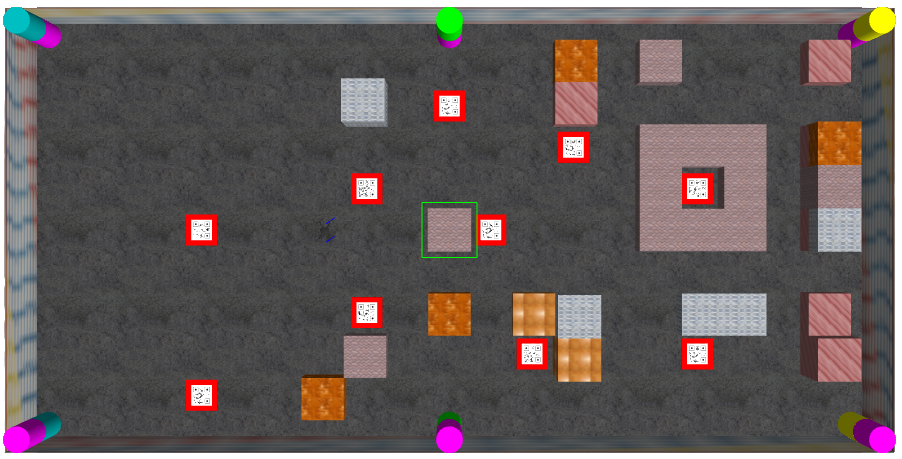
\includegraphics[width=\textwidth]{Images/fig18-gazebo-environment.png}
\caption{Gazebo simulated environment.}
\label{fig:chapter3:env:gazebo}
\end{figure}
The drone is placed at coordinates $(-3;0)$, and can be depicted in the figure as the green circle in the middle right. As mentioned before, the poles have a different combination of colors, where two poles have not the same combination. The markers, are QR codes framed in red, while obstacles are brown and gray boxes around the environment. The walls are made of a net-like material distinguishable from the obstacles, while the floor is a pavement-like material.

\section{Simulated Experiments}
\label{sec:chapter3:simulation}

\subsection{Procedures}
\label{subsec:chapter3:simulation:procedures}

\subsection{Results}
\label{subsec:chapter3:simulation:results}

%\section{Empirical Results ?}
%\label{sec:chapter3:empirical}
%
%\subsection{Procedures}
%\label{subsec:chapter3:empirical:procedures}
%
%\subsection{Results}
%\label{subsec:chapter3:empirical:results}